% \documentclass[handout]{beamer}
\documentclass{beamer}

%\setbeamercovered{dynamic}

\definecolor{nupurple}{RGB}{78, 42, 132}
\usetheme{Madrid}
\usecolortheme[named=nupurple]{structure}
% \useinnertheme{rounded}
% \useinnertheme[shadow]{rounded}

%\usetheme{Boadilla} 
\usefonttheme{serif}


%\usetheme{Darmstadt}
%\usefonttheme[onlylarge]{structurebold}
\setbeamerfont*{frametitle}{size=\normalsize,series=\bfseries}
\setbeamertemplate{navigation symbols}{}
\setbeamertemplate{footline}[frame number]

%\setbeamercovered{transparent}

\usepackage{xspace}
\usepackage{xcolor}
\usepackage{tikz}
\usepackage{lmodern}
\usepackage[english]{babel}
\usepackage[latin1]{inputenc}
\usepackage{times}
\usepackage[T1]{fontenc}
\usepackage{amsmath,amsthm,amssymb}
\usepackage{graphicx}
\usepackage{mathrsfs}
%\usepackage{caption}
%\usepackage{subcaption}
\usepackage{color}
\usepackage{environ}
\usepackage{mathtools}

\AtBeginSubsection[]{

  \frame<beamer>{

    \frametitle{Outline}

    \tableofcontents[currentsection,currentsubsection]

  }

}

\def\P{{\cal P}}
\def\si{\bar{\sigma}}
\def\E{{\cal E}}
\def\LL{{\cal L}}
\def\FF{{\cal F}}
\def\SS{{\cal S}}
\def\C{{\cal C}}
\def\H{{\cal H}}
\def\X{{\cal X}}
\def\Y{{\cal Y}}
\def\A{{\cal A}}
\def\B{{\cal B}}
\def\vX{\boldsymbol{X}}
\def\vY{\boldsymbol{Y}}
\def\vZ{\boldsymbol{Z}}
\def\O{{\cal O}}
\def\M{{\cal M}}
\def\I{{\cal I}}
\def\eps{{\varepsilon}}
\def\ch{{\mbox{\rm ch}\hspace{0.4mm}}}
\def\sh{{\mbox{\rm sh}}}
\def\th{{\mbox{\rm th}}}
\def\Av{{\mbox{\rm{Av}}}}
\def\n{\noindent}
\def\bbe{\vskip .15pc\hangindent=.5pc\hangafter=1}
\def\la{{\Bigl\langle}}
\def\ra{{\Bigr\rangle}}
\def\goin{\to\infty}
\def\qed{\hfill\break\rightline{$\bbox$}}

\newcommand{\ow}{\overline{w}}
\newcommand{\ou}{\overline{u}}
\newcommand{\ov}{\overline{v}}
\newcommand{\e}{\mathbb{E}}
\newcommand{\p}{\mathbb{P}}
\newcommand{\Reals}{\mathbb{R}}
\newcommand{\Natural}{\mathbb{N}}
\newcommand{\calA}{\mathcal{A}}
\newcommand{\F}{{\cal F}}
\newcommand{\veps}{\vec{\varepsilon}}
\newcommand{\vsi}{\boldsymbol{\sigma}}
\newcommand{\vrho}{{\boldsymbol{\rho}}}
\newcommand{\vbeta}{\vec{\beta}}
\newcommand{\vtau}{\boldsymbol{\tau}}
\newcommand{\veta}{\vec{\beta}}
\newcommand{\vx}{\mathbf{x}}
\newcommand{\vy}{\mathbf{y}}
\newcommand{\vz}{\mathbf{z}}
\newcommand{\vw}{\boldsymbol{w}}
\newcommand{\vW}{\boldsymbol{W}}
\newcommand{\Exval}[1]{\mathbb{E}#1}
\newcommand{\prob}[1]{\mathbb{P}(#1)}
\newcommand{\Prob}[1]{\mathbb{P}\{#1\}}
\newcommand{\bigProb}[1]{\mathbb{P}\Bigl\{#1\Bigr\}}
\newcommand{\bigprob}[1]{\mathbb{P}\left(#1\right)}
\newcommand{\showcite}[1]{\ensuremath{\stackrel{\textnormal{#1}}{\textnormal{\cite{#1}}}}}
\newcommand{\indi}{\ensuremath{\boldsymbol 1}}
\newcommand{\bB}{\mathbf{B}}
\newcommand{\bW}{\mathbf{W}}
\newcommand{\bu}{\mathbf{u}}
\newcommand{\bv}{\mathbf{v}}
\newcommand{\bF}{\mathcal{F}}
\newcommand{\bC}{\mathcal{C}}
\newcommand{\bL}{\mathcal{L}}
\newcommand{\bX}{\mathcal{X}}
\newcommand{\bY}{\mathcal{Y}}
\newcommand{\bZ}{\mathcal{Z}}
\newcommand{\lovasz}{{Lov\'asz}\xspace}
\newcommand{\ki}{\mathbf{Ker}_{\mathbf{I}}}
\newcommand{\ko}{\mathbf{Ker}_{\mathbf{O}}}
\newcommand\norm[1]{\left\lVert#1\right\rVert}

\newcommand{\Pp}{\mathcal{P}}
\newcommand{\s}{\boldsymbol{\sigma}}
\newcommand{\ii}{\iota}
\newcommand{\bt}{\boldsymbol{t}}
\DeclareMathOperator*{\argmax}{arg\,max}
\DeclareMathOperator*{\argmin}{arg\,min}


\newtheorem{proposition}{\bf Proposition}
\newtheorem{condition}{\bf Condition}
\NewEnviron{resizealign}{\sbox0{\let\notag=\relax
    $\begin{matrix}\displaystyle\BODY\end{matrix}$}%
  \sbox1{$(\theequation)$}%
  \sbox2{\parbox{\dimexpr \wd0 + 2\wd1}%
    {\begin{align}\BODY\end{align}}}% for testing
  \noindent\resizebox{\textwidth}{!}{\usebox2}%
}

\title{Ph.D. Thesis Defense}
\subtitle{Generalized t-SNE and Beyond: Probabilistic Methods for Dimensionality Reduction, Combinatorial Optimization, and Machine Learning}
\author[Yi Gu]{Yi Gu \texorpdfstring{\\}{} Advisor: Antonio Auffinger}

\institute{Department of Mathematics, Northwestern University}


\date{June 6, 2025}
\begin{document}

\frame{\titlepage}

%\section[Outline]{}
\begin{frame}\frametitle{Agenda}
  This thesis defense is about probabilistic algorithms along with the problems they aim to tackle.
  \begin{itemize}
    \item[$\bullet$] Two basic problems: Dimensionality and Dependence
    \item[$\bullet$] Dimensionality Reduction and t-SNE
    \item[$\bullet$] Dependence, Probabilistic Graphic Models and \lovasz Local Lemma
    \item[$\bullet$] Autoencoder and Variational Factor Analysis
  \end{itemize}
\end{frame}

\begin{frame}
  \frametitle{Challenges from high-dimensional data}
  Dimensionality has been with us since the dawn of time. It refers to different aspects of the information. The scale of dimensionality drastically increases during the modern era because of advancements in mathematics and computer science.
  \begin{itemize}
    \item[$\bullet$] Increasing dimensionality means we can store more data, even the raw information of the process we aim to analyze.
    \item[$\bullet$] However, it does not mean we are automatically able to extract insights from the data.
  \end{itemize}
\end{frame}

\begin{frame}
  \frametitle{Curse of dimensionality}
  \textbf{The curse of dimensionality}: a series of phenomena that arises in high-dimensional spaces that are usually not present or prominent in low-dimensional settings.

  \vspace{1em}
  Example: The volume of a hypercube gets concentrated in its corners. Let $C_d$, $S_d$ be the volume of the hypercube and hypersphere respectively.
  \begin{align}
    \lim_{d \to \infty} \frac{S_d}{C_d} = \lim_{d \to \infty} \frac{\pi^{d/2}}{d2^{d-1}\Gamma(d/2)} = 0.
  \end{align}
  %mention data points being in corners will increase the sparsity of the data.
\end{frame}

\begin{frame}
  \frametitle{Curse of dimensionality (cont.)}
  Example: the distribution of distance between uniformly distributed points is concentrated in high-dimensional spaces.
  \begin{figure}[ht]
    \centering
    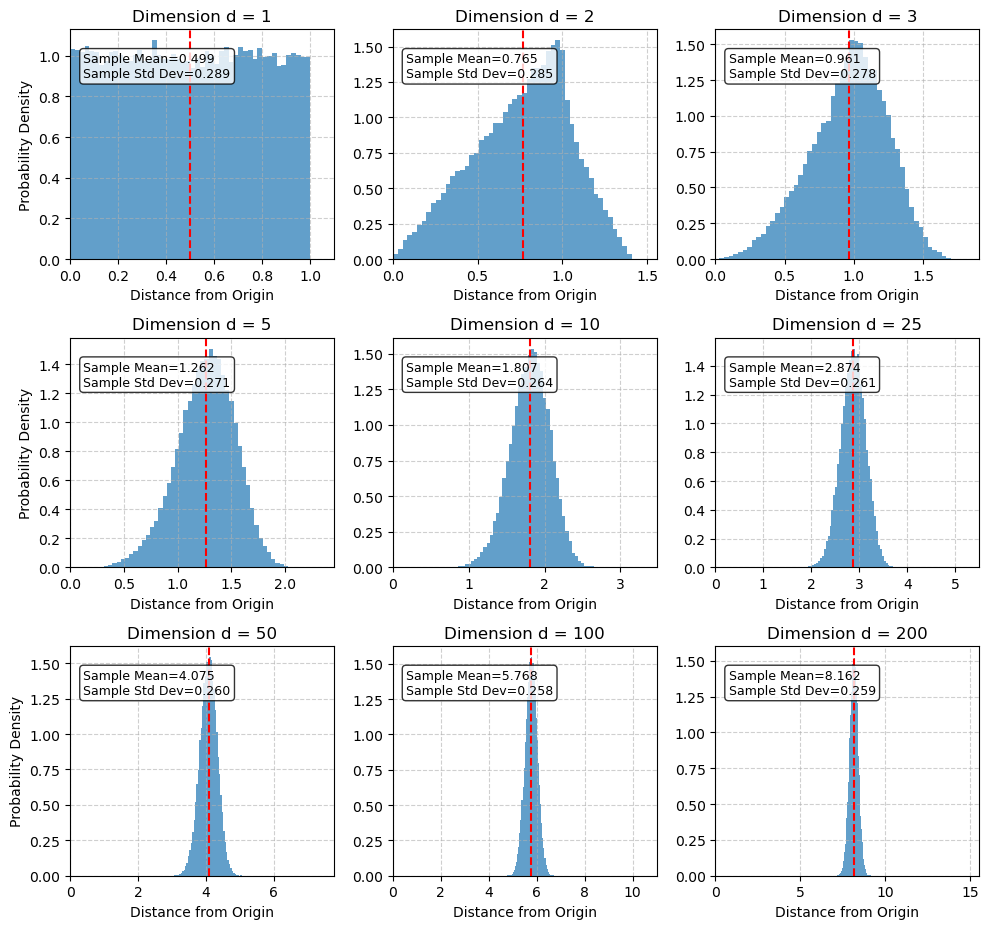
\includegraphics[width=7cm]{concentration_distance_hypercube.png}
  \end{figure}
  %mention two things: first distance becomes less informative and effective in terms of finding signals in the information; second, the Hughes phenomenon will appear and introduce overfitting. To achieve the same level of results we will need more data points.
\end{frame}

\begin{frame}
  \frametitle{Overview of t-SNE}
  t-distributed Stochastic Neighbor Embedding (t-SNE) is an algorithm that find a low-dimensional representation of high-dimensional data.

  \vspace{1em}
  $d,s \geq 2$ with $d>s$, and $n \geq 1$.
  \begin{itemize}
    \item[$\bullet$] \textbf{Input}: $X_1, \cdots, X_n \in \mathbb{R}^d$ the original data points.
    \item[$\bullet$] \textbf{Output}: $Y_1, \cdots, Y_n \in \mathbb{R}^s$ the low-dimensional representation.
  \end{itemize}

  \vspace{1em}
  Overall idea: KL-divergence (relative entropy) can be used to measure the difference between two distributions. t-SNE construct two distributions from both input and initial output data points, then minimize the KL-divergence by adjusting the output.
  %We cannot directly compare two collections of points in different dimensions, so we construct two distributions as a bridge.
\end{frame}

\begin{frame}
  \frametitle{The concept of kernels}
  \begin{definition} [Generalized Input Kernel] \label{def:input_kernel}
    The input kernel $\ki(x,y,\sigma): \mathbb{R}^d  \times \mathbb{R}^d \to \mathbb{R}^+$ is a function of the input data points and parameter $\sigma$ such that for any $x,y \in \mathbb{R}^d$ and $\sigma > 0$,
    \begin{color}{nupurple}
      \begin{align}
        \ki(x,y,\sigma)=\ki(y,x,\sigma).
      \end{align}
    \end{color}
  \end{definition}
  \begin{definition} [Generalized Output Kernel] \label{def:output_kernel}
    The output kernel $\ko(z,w):\mathbb{R}^s \times \mathbb{R}^s \to \mathbb{R}^+$ is a function of the output data points such that for any $z,w \in \mathbb{R}^s$,
    \begin{color}{nupurple}
      \begin{align}
        \ko(z,w)=\ko(w,z).
      \end{align}
    \end{color}
  \end{definition}
\end{frame}

\begin{frame}
  \frametitle{The concept of kernels(cont.)}
  Construct probability distributions from the input kernels:
  \begin{align}
    p_{j|i} = \frac{\ki(X_i,X_j,\sigma_i)}{\sum_{k \neq i} \ki(X_i,X_k,\sigma_i)}, \quad p_{ij} = \frac{p_{j|i} + p_{i|j}}{2n}.
  \end{align}
  %Say that we will get to the meaning of $\sigma_i$ right after.
  For output kernels:
  \begin{align}
    q_{ij} = \frac{\ko(Yi,Yj)}{\sum_{k \neq l}\ko(Y_k,Y_l)}.
  \end{align}
  Original t-SNE can be recovered by letting
  \begin{align}
    \ki(x,y,\sigma)=\exp\left(-\frac{||x-y||^2}{2\sigma^2}\right), \quad \ko(z,w)=\frac{1}{1+||z-w||^2}.
  \end{align}
\end{frame}

\begin{frame}
  \frametitle{The concept of perplexity}
  Recall
  \begin{align}
    p_{j|i} = \frac{\ki(X_i,X_j,\sigma_i)}{\sum_{k \neq i} \ki(X_i,X_k,\sigma_i)}.
  \end{align}
  $\sigma_i$ satisfies that for each $i = 1, \dots, n$,
  \begin{align}
    -\sum_{j = 1, j \neq i}^n p_{j|i} \log p_{j|i} = \log \textbf{Perp} =: \log (n \rho), \rho \in (0,1).
  \end{align}
  \textbf{Intuition}: $\sigma_i$ is the zoom slide bar for the input data points.
  %If a point is far away from others, than all other points do not make much difference and thus information gets compressed and lost. Perplexity is created to prevent that.
\end{frame}

\begin{frame}
  \frametitle{Algorithm setup}
  \begin{itemize}
    \item [$\bullet$] \textbf{Input}: $X_1, \cdots, X_n \in \mathbb{R}^d$ $\Longrightarrow$ $p_{ij}$.
    \item [$\bullet$] \textbf{Output}: $Y_1, \cdots, Y_n \in \mathbb{R}^s$ $\Longrightarrow$ $q_{ij}$.
    \item [$\bullet$] \textbf{Variables Involved}: $p_{ij}$ are fixed. $q_{ij}$ can be changed and is a function of $Y_i$ and $Y_j$.
    \item [$\bullet$] \textbf{Loss Function (Goal)}: minimize the KL-divergence:
          \begin{align}
            L_{n,\rho}(X,Y) = \sum_{1 \leq i \neq j \leq n} p_{ij} \log \left(\frac{p_{ij}}{q_{ij}}\right).
          \end{align}
    \item [$\bullet$] \textbf{End Result}:
          \begin{align}
            Y^* = \argmin_{Y \in (\mathbb{R}^s)^n}L_n(X,Y).
          \end{align}
  \end{itemize}
\end{frame}

\begin{frame}
  \frametitle{Some extra notations}
  \textbf{Continuous version of the entropy:}

  \begin{resizealign}
    F_{\rho,\mu}(x,\sigma) = \int \frac{\ki(x,x',\sigma)}{\int \ki(x,x',\sigma)d\mu(x')} \log \left(\frac{\ki(x,x',\sigma)}{\int \ki(x,x',\sigma)d\mu(x')}\right) d\mu(x') + \log \rho.
\end{resizealign}

$\sigma^*_{\rho,\mu} : \mathbb{R}^d \to \mathbb{R}$ the unique solution of the equation
\begin{align}
    F_{\rho,\mu}(x,\sigma) = 0.
\end{align}
$\sigma_i$ serves the anchor point of distributions induced by the input data. $\sigma^*_{\rho,\mu}$ is its asymptotic limit.
\end{frame}

\begin{frame}
  \frametitle{Some extra notations (cont.)}
\textbf{Continuous version of induced probability distributions:}

\vspace{1em}
$\psi: \mathbb{R}^d \to \mathbb{R}$ be a given function and $p_{\psi}: \mathbb{R}^d \times \mathbb{R}^d \to \mathbb{R}$ be defined by
\begin{align}
    p_{\psi}(x,x') = \frac{1}{2}\left( \frac{\ki(x,x',\psi(x))}{\int \ki(x,x',\psi(x))d\mu(x')} + \frac{\ki(x,x',\psi(x'))}{\int \ki(x,x',\psi(x'))d\mu(x)}\right).
\end{align}

$q: \mathbb{R}^s \times \mathbb{R}^s \to \mathbb{R}$ be given by
\begin{align}
    q(y,y') = \frac{\ko(y,y')}{\iint \ko(y,y')d\mu(y) d\mu(y')}.
\end{align}
\end{frame}

\begin{frame}
  \frametitle{Some extra notations (cont.)}
\textbf{Continuous version of the loss function:}
\begin{align}
    I_{\rho}(\mu) = \iint p_{\sigma^*_{\rho,\mu}}(x,x') \log\left(\frac{p_{\sigma^*_{\rho,\mu}}(x,x')}{q(y,y')}\right) d\mu(x,y) d\mu(x',y').
\end{align}
Recall $\mu_X \in \mathcal{M}(\mathbb{R}^d)$ is an arbitrary given probability measure. We set $\mathcal{P}_X$ to be the set of probability measures on $\mathbb{R}^d \times \mathbb{R}^s$ whose marginal coincides with $\mu_X$. Formally speaking,
\begin{align}
    \mathcal{P}_X := \{\mu \in \mathcal{M}(\mathbb{R}^d \times \mathbb{R}^s): \text{the $\mathbb{R}^d$ marginal of $\mu$ is $\mu_X$}\}.
\end{align}
Lastly, define
\begin{resizealign}
    \tilde{\mathcal{P}}_X := \left\{ \mu \in \mathcal{P}_X: \int (p_{\sigma^*_{\rho,\mu}}(x,x')-q(y,y'))\frac{\frac{\partial}{\partial y}\ko{(y,y')}}{\ko{(y,y')}} d\mu(x',y') = 0,\mu(x,y)\text{-a.e.}\right\}.
\end{resizealign}
\end{frame}

\begin{frame}
  \frametitle{Conditions for kernels}
  \begin{condition}[Input Kernel Conditions] \label{input_kernel_conditions}
    Let $w: \mathbb{R}_{\geq 0} \to \mathbb{R}_{\geq 0}$ be a fixed function. The input kernel has the form of
    \begin{align} \label{tsne:input_kernel}
        \ki(x,x',\sigma) = \exp(-w(\sigma\norm{x-x'}^{\theta}))
    \end{align}
    Here, $\theta>0$ is a fixed constant. $w$ satisfies:

    1. $\forall t \geq 0$, $w'(t)>0$. $\lim_{t \to \infty} w(t) = \infty$.

    2. $w'(t)+tw''(t) \geq 0$ for all $t \geq 0$.

    3. The following integral converges:
    \begin{align}
        \int_0^{\infty} t^{d-1} w(t^{\theta}) \exp(-w(t^{\theta}))dt < \infty.
    \end{align}
\end{condition}
Since the all probability masses are normalized, we can assume without loss of generality that $w(0)=0$ from now on.
\end{frame}

\begin{frame}
  \frametitle{Conditions for kernels}
\begin{condition}[Output Kernel Conditions] \label{output_kernel_conditions}
    The output kernel depends only on the distance between two output data points $y$ and $y'$. In particular, $\ko(y,y') = k (\norm{y-y'})$ and:

    1. $k: \mathbb{R}_{\geq 0} \to \mathbb{R}^+$ is decreasing and bounded.

    2. $\ko$ satisfies
    \begin{align}
        \iint_{(0,\infty)^2} \ko(y,y') dy dy' < \infty.
    \end{align}

    3. $k$ has bounded derivative.

    4. $k'(0) = 0$.
\end{condition}
\end{frame}

\begin{frame}
  \frametitle{Main results}
  \begin{theorem} \label{tsne:main_theorem_1}
    Assume $\mu_X$ has a continuous density $f(x)$ and compact support. Let $X_i \in \mathbb{R}^d$ be i.i.d random variables with probability measure $\mu_X$. If condition \ref{input_kernel_conditions} and condition \ref{output_kernel_conditions} hold, then for any $\rho \in (0,1)$,
    \begin{align}
        \lim_{n \to \infty} \inf_Y L_{n,\rho}(X,Y) = \inf_{\mu \in \tilde{\mathcal{P}}_X} I_{\rho}(\mu).
    \end{align}
    Moreover, there exist a measure $\mu^*$ and a sub-sequence $\{n_k\}$ such that $\mu_{n_k} \to \mu^*$ weakly and $I_{\rho}(\mu^*) = \inf_{\mu \in \tilde{\mathcal{P}}_X} I_{\rho}(\mu)$.
\end{theorem}
\begin{theorem} \label{tsne:main_theorem_2}
    Under the same assumptions of theorem \ref{tsne:main_theorem_1}, $\mu^*$ has compact support.
\end{theorem}
\end{frame}

\begin{frame}
  \frametitle{Interpretation}
\end{frame}

\begin{frame}
  \frametitle{Structure of proofs}
\end{frame}

\begin{frame}
  \frametitle{Existence and Uniqueness of $\sigma^*$}
\end{frame}

\begin{frame}
  \frametitle{The problems of dependence}
\end{frame}

\begin{frame}
  \frametitle{Probabilistic Graphical Models}
\end{frame}

\begin{frame}
  \frametitle{Markov Random Fields}
\end{frame}
% \begin{frame}\frametitle{Parisi measures}
% 	\noindent Given a (random) function 
% \begin{color}{blue}	
% 	$$ \H: \Sigma \to \mathbb R $$
% \end{color}	
% and $E \in \mathbb R$, what can we say about the level sets
% \begin{color}{blue}	
% $$ \mathcal L (E) := \{ \sigma \in \Sigma : \H(\sigma) = E  \}? $$
% \end{color}
% \end{frame}
\end{document}

